\documentclass[12pt,a4paper,twocolumn]{article}
\usepackage{graphicx}
\title{Probability and Random Variables Assignment}
\author{Maharshi Kadeval}
\date{29 March 2022}

\begin{document}

\maketitle

Q8c)\\
Using ruler and compass only, construct a $\bigtriangleup$ABC such that BC = 5 cm\\
and AB = 6.5 cm and $\angle$ABC = 120°\\
(i) Construct a circum-circle of $\bigtriangleup$ABC\\
(ii) Construct a cyclic quadrilateral ABCD, such that D is equidistant\\
from AB and BC.\\\\
SOLUTION:

(i)
\begin{figure}[!h]
\begin{center}
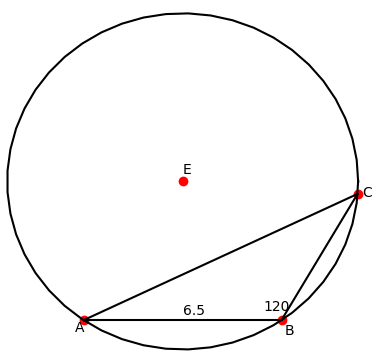
\includegraphics[scale=0.58]{fig1.png}\\
\end{center}
\end{figure}
\\
center of the circumcircle is the point of intersection of the perpendicular bisectors of AB and BC.

\pagebreak
(ii)
\begin{figure}[!h]
\begin{center}
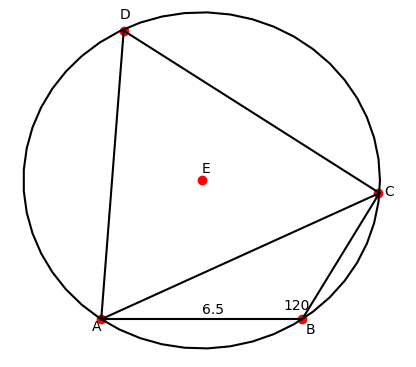
\includegraphics[scale=0.6]{fig2.png}\\
\end{center}
\end{figure}
\\
the point D of the cyclic quadrilateral ABCD is the point of intersection of the angle 
bisectors of AB and BC and the circumcircle.
\end{document}
